\newcolumntype{+}{>{\global\let\currentrowstyle\relax}}
\newcolumntype{^}{>{\currentrowstyle}}
\newcommand{\rowstyle}[1]{\gdef\currentrowstyle{#1}%
#1\ignorespaces
}

\newcommand{\specialcell}[2][c]{%
  \begin{tabular}[#1]{@{}c@{}}#2\end{tabular}}

\chapter{Experiments and Results}
\label{sec:exp}

The experiments and results presented in this section used the FPGA Atlys board and a desktop computer that has an i7 CPU 950 at 3.07 GHz, 16 GB of RAM, and runs Ubuntu 64-bit. Due to hardware and timing issues with the DDR RAM on the FPGA board, the board was unable to hold all of the data for both images. Part of the rows of both images were sent to the FPGA board from the computer. The board processed the data and send the disparity values back to the computer. The computer then provide the board with the next set of data and so on until the entire disparity map was created. This was used to test the quality and accuracy of the disparity maps from the FPGA implementation in comparison to computer implementations. The transfer time of sending both images to the FPGA board and getting back the disparity map was not a real-time solution since it took around 20 seconds to complete the whole process. To test for the maximum possible frames per second the SAD wrapper perform at, testbench simulations were used to obtain the time it should take to produce a disparity map on the board at a 100 MHz clock. The Atlys board has a 100 MHz clock on it, so that determined the clock cycle of 10 ns in the testbench simulations. However, for the experiments that produced the disparity image maps where the image data came from the computer to the board, a 48 MHz clock was used, which is the clock frequency of the FPGALink. This was done in order to keep the input data in sync with the SAD wrapper.

\section{Window Size Selection}
\label{sec:windowSize}

The size of the window (e.g. 9x9 pixels) affects the quality of the disparity map (see Figure~\ref{fig:tsukubaWinSize}) and the number of computations required to create the disparity map. The 3x3 window size in Figure~\ref{fig:tsukuba3x3} is processed the fastest out of the window sizes shown since each SAD calculation only has 9 pairs of pixels. The 13x13 window in Figure~\ref{fig:tsukuba13x13} has 169 pairs of pixels, which will require 160 more calculations per SAD value. However, the 13x13 window has the least amount of noise in its disparity map, but it loses some detail as shown by comparing the neck of the lamp in the foreground of the image compared to the lamp necks in the other images. Table~\ref{table:pixelCount} shows the number of pixels required for different window sizes with a disparity range of 16. The disparity values (1, 2, and 4) represent the number of pixels processed in parallel. The number of pixels show how many pixels are needed from the pair of images to calculate disparity values for the pixels processed in parallel (1, 2, and 4). As the window size gets larger, more resources are needed on the FPGA board. The 7x7 and 9x9 window sizes were used because they provided a good compromise on the amount of noise in the disparity maps and the amount of hardware resources required for implementation.

\begin{figure}
\begin{center}
	\begin{subfigure}{0.45\textwidth}
		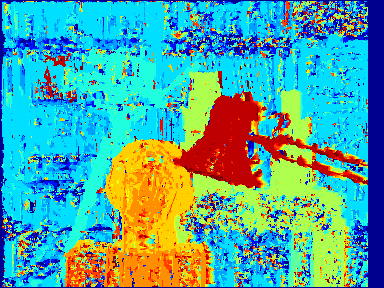
\includegraphics[width=\textwidth]{figures/sad_tsukuba_3x3_0-15.png}
		\caption{SAD 3x3 Window Disparity Map}
		\label{fig:tsukuba3x3}
	\end{subfigure}
	\begin{subfigure}{0.45\textwidth}
		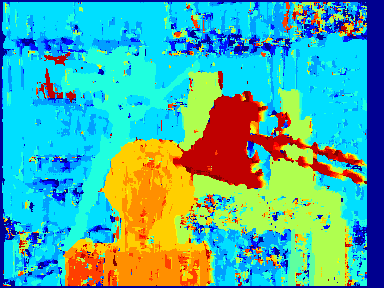
\includegraphics[width=\textwidth]{figures/sad_tsukuba_5x5_0-15.png}
		\caption{SAD 5x5 Window Disparity Map}
		\label{fig:tsukuba5x5}
	\end{subfigure}
	\\
	\begin{subfigure}{0.45\textwidth}
		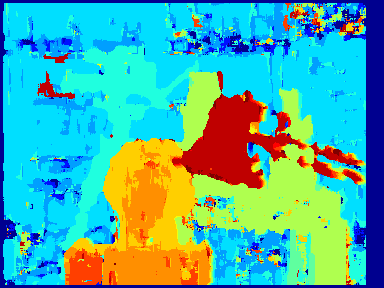
\includegraphics[width=\textwidth]{figures/sad_tsukuba_7x7_0-15.png}
		\caption{SAD 7x7 Window Disparity Map}
		\label{fig:tsukuba7x7}
	\end{subfigure}
	\begin{subfigure}{0.45\textwidth}
		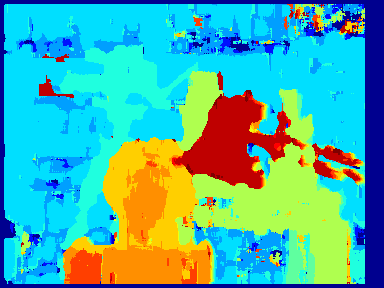
\includegraphics[width=\textwidth]{figures/sad_tsukuba_9x9_0-15.png}
		\caption{SAD 9x9 Window Disparity Map}
		\label{fig:tsukuba9x9}
	\end{subfigure}
	\\
	\begin{subfigure}{0.45\textwidth}
		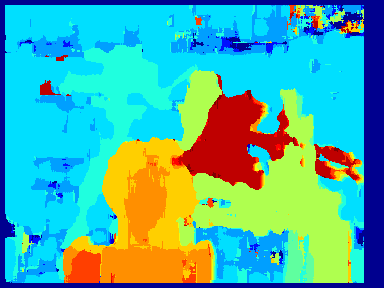
\includegraphics[width=\textwidth]{figures/sad_tsukuba_11x11_0-15.png}
		\caption{SAD 11x11 Window Disparity Map}
		\label{fig:tsukuba11x11}
	\end{subfigure}
	\begin{subfigure}{0.45\textwidth}
		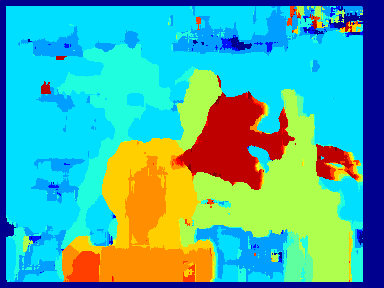
\includegraphics[width=\textwidth]{figures/sad_tsukuba_13x13_0-15.png}
		\caption{SAD 13x13 Window Disparity Map}
		\label{fig:tsukuba13x13}
	\end{subfigure}
	\captionfonts
	\caption{Window size comparisons for disparity maps~\cite{matlab} of the Tskukuba image pair~\cite{middlebury}.}
	\label{fig:tsukubaWinSize}
\end{center}
\end{figure}

\begin{table}
\begin{center}
	\begin{tabular}{| p{1.7cm} | p{2.5cm} | p{2.7cm} | p{2.7cm} | p{2.7cm} |}
		\hline
		\rowstyle{\bfseries} Window Size & 
		\rowstyle{\bfseries} \# of pixels/ window & 
		\rowstyle{\bfseries} \# of pixels/ disparity value &
		\rowstyle{\bfseries} \# of pixels/2 disparity values & 
		\rowstyle{\bfseries} \# of pixels/4 disparity values %& 
		%\rowstyle{\bfseries} \# of MUXCYs, out of 13,644
		\tabularnewline
		\hline
		3x3 & 9 & 108 & 114 & 126
		\tabularnewline
		\hline
		5x5 & 25 & 200 & 210 & 230
		\tabularnewline
		\hline
		\rowstyle{\bfseries} 7x7 & 
		\rowstyle{\bfseries} 49 & 
		\rowstyle{\bfseries} 308 & 
		\rowstyle{\bfseries} 322 & 
		\rowstyle{\bfseries} 350
		\tabularnewline
		\hline
		\rowstyle{\bfseries} 9x9 & 
		\rowstyle{\bfseries} 81 & 
		\rowstyle{\bfseries} 432 & 
		\rowstyle{\bfseries} 480 & 
		\rowstyle{\bfseries} 486
		\tabularnewline
		\hline
		11x11 & 121 & 572 & 594 & 638
		\tabularnewline
		\hline
		13x13 & 169 & 728 & 754 & 806		
 		\tabularnewline
		\hline 
	\end{tabular}
	\captionfonts
	\caption{Number of 1 byte pixels need based on the window size and number of pixels processed in parallel for producing a number of disparity values simultaneously for a disparity range of 16.}
	\label{table:pixelCount}
\end{center}
\end{table}

\section{Resource Utilization on FPGA}
\label{sec:utilize}

The disparity range used to obtain the disparity value for each pixel affects the number of SAD entities and the number of minimum comparator entities required. Table~\ref{table:dispRange} shows the direct correlation between the disparity range and number of those entities needed. A lower disparity range of 8 requires fewer resources, but does not work well for objects that get close to the pair of cameras. A disparity range of 32 will give better results with objects that are closer; however, the resource requirements increase as well. The disparity range of 16 was used, since it provided a compromise of resource space to detectable object distance. For a disparity range of 16, Table~\ref{table:pixelInParallel} shows the amount of SAD entities and minimum comparators needed for processing different numbers of pixels in parallel. Processing 2 or 4 pixels in parallel allowed for the speed needed while allowing for a resource utilization size that fits on the Atlys board.

\begin{table}
\begin{center}
	\begin{tabular}{| p{2cm} | p{4cm} | p{5cm} |}
		\hline 
		\rowstyle{\bfseries} Disparity Range & 
		\rowstyle{\bfseries} \# of SAD entities/ pixel in parallel &
		\rowstyle{\bfseries} \# of Min Comp entities/ pixel in parallel
		\\ \hline
		8 & 8 & 7
		\\ \hline 
		\rowstyle{\bfseries} 16 & 
		\rowstyle{\bfseries} 16 & 
		\rowstyle{\bfseries} 15
		\\ \hline
		32 & 32 & 31
		\\ \hline 
	\end{tabular}
	\captionfonts
	\caption{Number of SAD calculation entities and minimum comparators entities needed per pixel processed in parallel based on the disparity range.}
	\label{table:dispRange}
\end{center}
\end{table}

\begin{table}
\begin{center}
	\begin{tabular}{| p{3cm} | p{3cm} | p{3cm} |}
		\hline 
		\rowstyle{\bfseries} \# of pixels in parallel & 
		\rowstyle{\bfseries} \# of SAD entities &
		\rowstyle{\bfseries} \# of Min Comp entities 
		\\ \hline
		1 & 16 & 15
		\\ \hline 
		\rowstyle{\bfseries} 2 & 
		\rowstyle{\bfseries} 32 & 
		\rowstyle{\bfseries} 30
		\\ \hline 
		\rowstyle{\bfseries} 4 & 
		\rowstyle{\bfseries} 64 & 
		\rowstyle{\bfseries} 60
		\\ \hline
		6 & 96 & 90
		\\ \hline 
	\end{tabular}
	\captionfonts
	\caption{Number of SAD calculation and minimum comparator entities needed based on the number of pixels processed in parallel for a disparity range of 16.}
	\label{table:pixelInParallel}
\end{center}
\end{table}

See Table~\ref{table:utilize} for resource utilization. The 7x7 window implementation actually uses more resources on the FPGA board than the 9x9 window implementation due to the amount of parallel calculations used in the SAD algorithm. There is still plenty of space on the board for other top level entity designs for this SAD module.

\begin{table}
\begin{center}
	\begin{tabular}{| p{1.9cm} | p{2.2cm} | p{2.5cm} | p{2.9cm} | p{2.7cm} |}
		\hline
		\rowstyle{\bfseries} Window Size & 
		\rowstyle{\bfseries} \# of pixels in parallel & 
		\rowstyle{\bfseries} SAD Alg. Parallelized & 
		\rowstyle{\bfseries} \# of Slice Registers, out of 54,576 &
		\rowstyle{\bfseries} \# of Slice LUTs, out of 27,288 %& 
		%\rowstyle{\bfseries} \# of occupied Slices, out of 6,822
		\tabularnewline
		\hline
		7x7 & 4 & No & 6,512 (11\%) & 12,297 (45\%) %& 3,267 (47\%) 
		\tabularnewline
		\hline 
		\rowstyle{\bfseries} 7x7 & 
		\rowstyle{\bfseries} 2 & 
		\rowstyle{\bfseries} Yes & 
		\rowstyle{\bfseries} 8,343 (15\%) & 
		\rowstyle{\bfseries} 17,631 (64\%) %& 5,712 (83\%) 
		\tabularnewline
		\hline 
		\rowstyle{\bfseries} 9x9 & 
		\rowstyle{\bfseries} 4 & 
		\rowstyle{\bfseries} No & 
		\rowstyle{\bfseries} 10,445 (19\%) & 
		\rowstyle{\bfseries} 19,082 (69\%) %& 4,355 (63\%)
		\tabularnewline
		\hline
		9x9 & 2 & No & 8,176 (14\%) & 15,658 (57\%) %& 3,471 (50\%)
		\tabularnewline
		\hline 
		9x9 & 1 & No & 6,947 (12\%) & 12,745 (46\%) %& 3,066 (44\%)
		\tabularnewline
		\hline 
	\end{tabular}
	\captionfonts
	\caption{Resource utilization on the FPGA Atlys board for the window implementations.}
	\label{table:utilize}
\end{center}
\end{table}

\section{Testbench Simulation}
\label{sec:testbench}

See Figure~\ref{fig:tb_9x9} and Figure~\ref{fig:tb_7x7} in Appendix~\ref{sec:appdxD} for the testbench simulations for the 9x9 window and 7x7 window implementations, respectively.

The signal h2fvalid\_i, near the top of the figures, went high when image data is sent to the SAD wrapper. The first time h2fvalid\_i went high until the second time it went high was when the initial rows were given to the wrapper up to when the initial disparity values were produced. A cycle began afterwards where h2fvalid\_i would go high for several clock cycles and then go low for several more clock cycles. The high section represented when the next row was sent to the wrapper while the low section represented the time it took to calculate the SAD values and produce the next disparity values. The wrapper has been designed to allow both the template image data and the search image data to be sent to the wrapper at the same time, thus reducing the amount of time taken to get all necessary data into the wrapper. When the signal f2hready\_i goes high, it means that the disparity values are being sent out of the wrapper.

\subsection{9x9 Window Implementation Runtime}
\label{sec:testbench9x9}

Based on the testbench simulation in Fig.~\ref{fig:tb_9x9} the simulated frames per second can be inferred for different image sizes. The simulation assumes the 100 MHz clock on the FPGA is used, which is the clock frequency used on the Atlys board. The clock cycle duration is therefore 10 ns long.

In the testbench simulation, the window size is 9x9 and 4 pixels are processed in parallel. The first section of the simulation includes the initial image data given to the SAD wrapper up to the point where that data's disparity values are returned. This section takes 3.35 us. After that, a constant cycle is produced, which includes the SAD wrapper taking in the next row and producing the next disparity values. This cycle takes 1.22 us. A 640x480 image has 307,200 pixels, which will produce a disparity map of 617x472, or 291,224 pixels. Disparity values are not produced for pixels where either the window would run off the image or where there is not enough room for the 16 SAD values to be calculated for the pixel. Since 4 pixels are processed in parallel, 291,224 pixels are divided by 4 pixels/iteration, giving 72,806 iterations. So, 72,805 iterations times 1.22 us/iteration plus 3.35 us (initial section, hence minus one on number of iterations) gives 88,826.67 us or approximately 0.0888 seconds per frame. Therefore, an image size of 640x480 can be processed at around 11.26 frames per second. Table~\ref{table:tb_9x9} shows the simulated frame rate for the image sizes used in this chapter.

\begin{table}
	\begin{center}
		\begin{tabular}{|c|c|c|c|c|}
			\hline 
				\rowstyle{\bfseries} Image & 
				\rowstyle{\bfseries} Image Width & 
				\rowstyle{\bfseries} Image Height & 
				\rowstyle{\bfseries} Sec/frame & 
				\rowstyle{\bfseries} Frames/sec
			\tabularnewline
			\hline 
			VmodCAM & 640 & 480 & 0.0888 & 11.26
			\tabularnewline
			\hline 
			Tsukuba & 384 & 288 & 0.0308 & 32.43
			\tabularnewline
			\hline 
			Venus & 434 & 383 & 0.0470 & 21.27
			\tabularnewline
			\hline 			
			\end{tabular}
		\captionfonts
		\caption{9x9 window for the testbench simulated runtime for the FPGA board for different image sizes.}
		\label{table:tb_9x9}
	\end{center}
\end{table}

\subsection{7x7 Window Implementation Runtime}
\label{sec:testbench7x7}

Based on the testbench simulation in Fig.~\ref{fig:tb_7x7} the simulated frame rate can be inferred for different image sizes. The simulation uses a clock cycle of 10 ns.

In the testbench simulation, the window size is 7x7 and 2 pixels are processed in parallel. The first section of the simulation includes the initial image data given to the SAD wrapper up to the point where that data's disparity values are returned. This section takes 1.78 us. After that, a constant cycle is produced allowing the SAD wrapper to get the next row and produce the next disparity values, which takes 0.42 us. A 640x480 image has 307,200 pixels, which will produce a disparity map of 619x474, which is 293,406 pixels. Disparity values are not produced for pixels that either the windows cannot fit on or there is not enough room for the 16 SAD values to be calculated for the pixel. Since 2 pixels are processed in parallel, 293,406 pixels is divided by 2 pixels/iteration, giving 146,703 iterations. So, 146,702 iterations times 0.42 us/iteration plus 1.78 us (initial section, hence minus one on number of iterations) gives 61,617.04 us or approximately 0.0616 seconds per frame. Therefore, an image size of 640x480 can be processed at around 16.23 frames per second. Table~\ref{table:tb_7x7} shows the simulated frame rate for the image sizes used in this chapter.

\begin{table}
	\begin{center}
		\begin{tabular}{|c|c|c|c|c|}
			\hline
				\rowstyle{\bfseries} Image & 
				\rowstyle{\bfseries} Image Width & 
				\rowstyle{\bfseries} Image Height & 
				\rowstyle{\bfseries} Sec/frame & 
				\rowstyle{\bfseries} Frames/sec
			\\ \hline 
			VmodCAM & 640 & 480 & 0.0616 & 16.23
			\\ \hline 
			Tsukuba & 384 & 288 & 0.0215 & 46.51
			\\ \hline 
			Venus & 434 & 383 & 0.0327 & 30.58
			\\ \hline 
		\end{tabular}	
		\captionfonts
		\caption{7x7 window for the testbench simulation runtime for the FPGA board for different image sizes.}
		\label{table:tb_7x7}
	\end{center}
\end{table}

\subsubsection{Pixel Parallelization}
\label{sec:7x7pixelParallel4}

The 7x7 window implementation used a parallelized SAD algorithm (see Section~\ref{sec:7x7window}). Due to the additional resources needed, only 2 pixels could be processed in parallel instead of 4. The reduced number of pixels in parallel is made up for by the speed up of the SAD algorithm. A variant of 7x7 window implementation was used that processed 4 pixels in parallel (the Atlys board was unable to support more) and used the SAD algorithm implementation similar to the 9x9 window implementation (see Section~\ref{sec:9x9window}). For a 640x480 image pair, the testbench simulation of the variant 7x7 implementation was shown to perform at a rate of 15.15 frames per second, which is slightly slower than the 16.23 frames per second the main 7x7 implementation had. The main 7x7 implementation was used for its higher frame rate.

\subsection{Frame Rate}
\label{sec:frameRate}

The smaller the image size, the higher the frame rate, as shown in Figure~\ref{fig:frameRate}. Once the number of pixels in an image goes below 180,000 for the 7x7 window implementation or 140,000 for the 9x9 window implementation, the frame rate approaches 30 frames per second. For robots, a frame rate of 10 should be sufficient for most tasks. Both the 9x9 and 7x7 window implementations were shown be above 10 frames per second for an image size of 640x480.

\begin{figure}[h]
	\begin{center}
		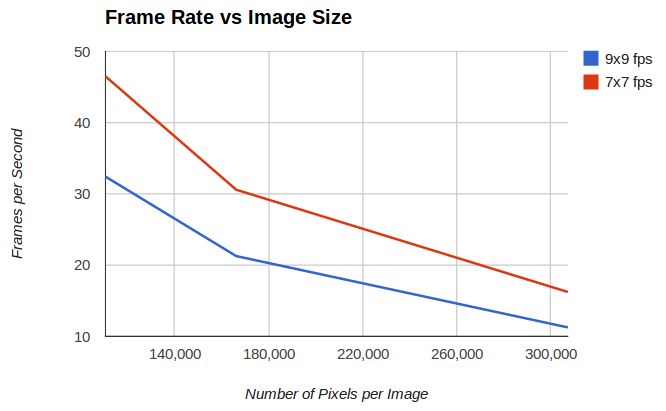
\includegraphics[width=100mm]{figures/frameRate.png}
		\captionfonts
		\caption{Frame rate comparison of different image sizes.}
		\label{fig:frameRate}
	\end{center}
\end{figure}

\section{FPGA Clock Cycle Runtimes}

\begin{subequations}
\begin{align} 	\label{eq:clockCycles}
	height = 288 	\qquad & \text{(image height)}\\
	width = 384 	\qquad & \text{(image width)}\\
	winSize = 9	 	\qquad & \text{(9x9 window size)}\\
	dispRange = 16 	\qquad & \text{(disparity range 0-15)}\\
	parPix = 4 		\qquad & \text{(pixels processed in parallel)}\\
	sadCyc = 82		\qquad & \text{(\# of cycles for SAD algorithm)}\\
	minCyc = 4		\qquad & \text{(\# of cycles for Min. comparator)}\\
	dispH = 280 &= height - (winSize - 1) \\
	lessPix = 23 &= (dispRange-1) + (winSize-1) \\
	dispW = 360 &= (width-lessPix) - (width-lessPix) \% parPix \\
	dispPixels = 100,800 &= dispH * dispW \\
	baseIters = 25,200 &= dispPixels / parPix \\
	colAdd = 89 &= dispWidth / parPix - 1 \\
	addIters = 712 &= colAdd * (winSize-1) \\
	totIters = 25,912 &= basIters + addIters \\
	sadTotCyc = 2,124,784 &= sadCyc * totIters \\
	minTotCyc = 103,648 &= minCyc * totIters \\
	extraCyc = 52,824 &= totIters * 2 \\
	totClkCyc = 2,306,168 &= sadTotCyc + minTotCyc + extraCyc
\end{align}
\end{subequations}


%\begin{subequations}
%\begin{align} 	\label{eq:clockCycles}
%	height = 288	&	\quad \text{(image height)}\\
%	width = 384 	&	\quad \text{(image width)}\\
%	winSize = 9	 	&	\quad \text{(9x9 window size)}\\
%	dispRange = 16 	&	\quad \text{(disparity range 0-15)}\\
%	parPix = 4 		&	\quad \text{(pixels processed in parallel)}\\
%	dispH &= height - (winSize - 1) \\
%	      &= 280	\nonumber \\
%	lessPix &= (dispRange-1) + (winSize-1) \\
%	dispW &= (width-lessPix) - (width-lessPix) \% parPix \\
%	dispW &= 360	\nonumber \\
%	dispPixels &= dispH * dispW \\
%			   &= 100,800 \nonumber \\
%	baseIters &= dispPixels / parPix \\
%			  &= 25,200 \nonumber \\
%	colAdd &= dispWidth / parPix - 1 \\
%	       &= 89 \nonumber \\
%	addIters &= colAdd * (winSize-1) \\
%			 &= 712 \nonumber \\
%	totIters &= basIters + addIters \\
%			 &= 25,912 \nonumber \\
%	sadCyc = 82	&	\quad \text{(\# of cycles for SAD algorithm)}\\
%	minCyc = 4		&	\quad \text{(\# of cycles for Min. comparator)}\\
%	sadTotCyc &= sadCyc * totIters \\
%			  &= 2,124,784 \nonumber \\
%	minTotCyc &= minCyc * totIters \\
%			  &= 103,648 \nonumber \\
%	totClkCyc &= sadTotCyc + minTotCyc \\
%			  &= 2,228,432 \nonumber
%\end{align}
%\end{subequations}


\begin{table}
	\begin{center}
		\begin{tabu}{| p{1.8cm} | p{2cm} | p{1,7cm} | p{1.7cm} | p{1.7cm} | p{1.5cm} | p{1.6cm} |}
			\hline
				\rowstyle{\bfseries} Image Size (HxW) & 
				\rowstyle{\bfseries} Disparity Image Size & 
				\rowstyle{\bfseries} Window Size & 
				\rowstyle{\bfseries} SAD Cycles & 
				\rowstyle{\bfseries} Min. Comp. Cycles &
				\rowstyle{\bfseries} Extra Cycles &
				\rowstyle{\bfseries} Total Clock Cycles			
			\\ \hline 
			288 x 384 & 280 x 360 & 9x9 & 2,124,784 & 103,648 & 51,824 & 2,306,168
			\\ \hline 
			288 x 384 & 282 x 362 & 7x7 & 416,976 & 208,488 & 521,220 & 1,198,806
			\\ \hline 
			288 x 384 & 282 x 360 & \specialcell{7x7\\(4 pix //)} & 1,295,700 & 103,656 & 51,828 & 1,477,098
			\\ \tabucline[2pt]{-} 
			
			383 x 434 & 375 x 408 & 9x9 & 3,202,756 & 156,232 & 78,116 & 3,476,162
			\\ \hline 
			383 x 434 & 377 x 412 & 7x7 & 631,136 & 315,568 & 788,920 & 1,814,516
			\\ \hline 
			383 x 434 & 377 x 412 & \specialcell{7x7\\(4 pix //)} & 1,972,150 & 157,772 & 78,886 & 2,248,251
			\\ \tabucline[2pt]{-}
			
			480 x 640 & 472 x 616 & 9x9 & 6,060,784 & 295,648 & 147,824 & 6,578,168
			\\ \hline 
			480 x 640 & 474 x 618 & 7x7 & 1,186,512 & 593,256 & 1,483,140 & 3,411,222
			\\ \hline 
			480 x 640 & 474 x 616 & \specialcell{7x7\\(4 pix //)} & 3,695,700 & 295,656 & 147,828 & 4,213,098
			\\ \hline
		\end{tabu}	
		\captionfonts
		\caption{Number of clock cycles counted when a pair of images were processed on the FPGA for the SAD algorithm and the minimum comparator .}
		\label{table:clockCount}
	\end{center}
\end{table}

\begin{table}
	\begin{center}
		\begin{tabu}{| p{1.8cm} | p{2cm} | p{2cm} | p{2cm} | p{2cm} | p{2cm} |}
			\hline
				\rowstyle{\bfseries} Window Size & 
				\rowstyle{\bfseries} Total Cycles & 
				\rowstyle{\bfseries} Sec/ Frame @ 48MHz & 
				\rowstyle{\bfseries} Sec/ Frame @ 100MHz & 
				\rowstyle{\bfseries} Frames/ Sec @ 48MHz &
				\rowstyle{\bfseries} Frames/ Sec @ 100MHz
			\\ \hline 
			9x9 & 2,306,168 & 0.04612 & 0.02306 & 21.68 & 43.36
			\\ \hline 
			7x7 & 1,198,806 & 0.02398 & 0.01199 & 41.71 & 83.42
			\\ \hline 
			\specialcell{7x7\\(4 pix //)} & 1,477,098 & 0.02954 & 0.0148 & 33.85 & 67.70
			\\ \tabucline[2pt]{-} 
			
			9x9 & 3,476,162 & 0.06952 & 0.03476 & 14.38 & 28.77
			\\ \hline 
			7x7 & 1,814,516 & 0.03629 & 0.01815 & 27.56 & 55.11
			\\ \hline 
			\specialcell{7x7\\(4 pix //)} & 2,248,251 & 0.04497 & 0.02248 & 22.24 & 44.48
			\\ \tabucline[2pt]{-}
			
			9x9 & 6,578,168 & 0.13156 & 0.06578 & 7.60 & 15.20
			\\ \hline 
			7x7 & 3,411,222 & 0.06822 & 0.03411 & 14.66 & 29.32
			\\ \hline 
			\specialcell{7x7\\(4 pix //)} & 4,213,098 & 0.08426 & 0.04213 & 11.87 & 23.74
			\\ \hline
		\end{tabu}	
		\captionfonts
		\caption{Frame rates that are possible for the number of clock cycles taken per image.}
		\label{table:clockCountFPS}
	\end{center}
\end{table}


\section{Test Image Pairs}
\label{sec:runtime}

In this section, FPGA disparity maps are compared to disparity maps created using C code. Part of the SAD algorithm implementation in C is shown in Appendix~\ref{sec:appdxE}. The C SAD version is performed completely in serial, so 1 pixel is processed at a time. The images the C version produced were used to compare disparity map quality and runtime of the algorithm. Python was used to convert the data in the grayscale image pairs into text files. Each row was separated by a new line. Each column was separated by a blank space. The C code read in the data from the text files, performed the SAD algorithm on the data, and wrote the disparity map data to a text file. The disparity map text file was read by a Python script and converted to a disparity map image. The time comparisons focused on the total time it took the SAD algorithm to run and disparity map data to be generated. Table~\ref{table:runtimeComp} shows the frame rate comparisons.

\begin{table}
	\begin{center}
		\begin{tabu}{|c|c|c|c|c|c|}
			\hline
				\rowstyle{\bfseries} Image & 
				\rowstyle{\bfseries} Window Size & 
				\rowstyle{\bfseries} Code & 
				\rowstyle{\bfseries} Sec/frame & 
				\rowstyle{\bfseries} FPS &
				\rowstyle{\bfseries} Speed up
			\\ \hline 
			Tsukuba & 7x7 & C & 0.1532 & 6.527 & 1
			\\ \hline 
			Tsukuba & 7x7 & VHDL & 0.0215 & 83.42 & 12.78
			\\ \tabucline[2pt]{-}
			Tsukuba & 9x9 & C & 0.2454 & 4.075 & 1
			\\ \hline 
			Tsukuba & 9x9 & VHDL & 0.0308 & 43.36 & 10.64
			\\ \tabucline[2pt]{-}
			Venus & 7x7 & C & 0.2327 & 4.297 & 1
			\\ \hline 
			Venus & 7x7 & VHDL & 0.0327 & 55.11 & 12.83
			\\ \tabucline[2pt]{-}
			Venus & 9x9 & C & 0.3776 & 2.648 & 1
			\\ \hline 
			Venus & 9x9 & VHDL & 0.0470 & 28.77 & 10.86
			\\ \hline 
		\end{tabu}	
		\captionfonts
		\caption{Tsukuba and Venus image pairs comparison runtimes for C code and FPGA testbench simulations. The disparity range is 16 for both.}
		\label{table:runtimeComp}
	\end{center}
\end{table}

\subsection{Data Overflows}
\label{sec:overflow}

The code for the hardware to be generated is designed in VHDL. The size of the data used for storing logic and values in hardware is defined during the coding process. In the SAD algorithm, it is possible for the SAD value to become much larger than the individual pixel values. For example, the pixel values range from 0 to 255, or 8 bits, while some SAD values could be over 4,095 and need to be stored in more than 12 bits. Most SAD values were under 4,096, so to account for those that were above it, the SAD algorithm use 14 bits to account for any values from 0 to 16,383. Figure~\ref{fig:overflow} shows what can happen when the data size allotted for the SAD algorithm is not large enough (i.e. only having 10 bits for storage). The data used is unsigned, so when it goes above the highest supported value, it goes back to 0 and continues from there.

Since most of the values were below 4,096, a measure was put in place in order to reduce the amount of bits needed during the minimum comparisons. If a SAD value was greater than 4,095, then 4,095 was returned for the calculated SAD because the greater the value, the less likely that search pixel is the correct corresponding one to the template pixel. In Figure~\ref{fig:tsukubaDispMap} and Figure~\ref{fig:venusDispMap}, the only noticeable difference in the C to FPGA comparisons is at the top of the images. The colors, warmer is closer and cooler is farther away, show that the top areas are thought to be closer than they actually are in the FPGA images. For a robot, it would be better to error on the side of thinking an object is closer than it actually is because the robot will be less prone to collide with the object. If a robot thought an object was farther away than it actually was, then the likelihood of collision would increase.

\begin{figure}[h]
	\begin{center}
		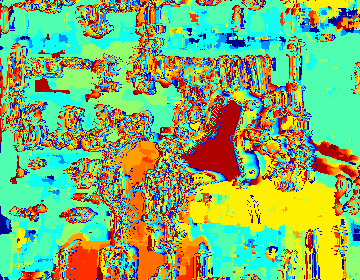
\includegraphics[width=80mm]{figures/tsukuba_disp9x9_2_sad_overflow.png}
		\captionfonts
		\caption{Data overflow for Tskukuba image pair~\cite{middlebury}.}
		\label{fig:overflow}
	\end{center}
\end{figure}

\subsection{Tsukuba}
\label{sec:tsukuba}

In Figure~\ref{fig:tsukubaL} and Figure~\ref{fig:tsukubaR}, the Tsukuba image pair is shown. Figure~\ref{fig:tsukubaDispMap} shows how the 7x7 window implementation is slightly noisier than the 9x9 window implementation. As discussed in Section~\ref{sec:overflow}, the only difference between the C implementation and the FPGA implementation is at the top of the disparity maps. This difference is caused by not having enough similarities between corresponding regions. It is possible for certain parts of an object in one image to be occluded in the image. This caused SAD values to be greater than normal. 

For Tsukuba, the FPGA version has a simulated runtime of 32.43 and 46.51 frames per second for the 9x9 and 7x7 window implementations, respectively, from Table~\ref{table:tb_9x9} and Table~\ref{table:tb_7x7}. For a speed comparison, the SAD algorithm was implemented in C since it is faster than Python. Python code handled the code for reading the images and creating the disparity map. As shown in Tbl.~\ref{table:runtimeComp}, the C code processed the images serially, which took 1.4128 seconds for the 9x9 window with a disparity range of 16. The 7x7 window implementation in C with a disparity range of 16 took 0.8849 seconds to complete.

\begin{figure}
\begin{center}
	\begin{subfigure}{0.45\textwidth}
		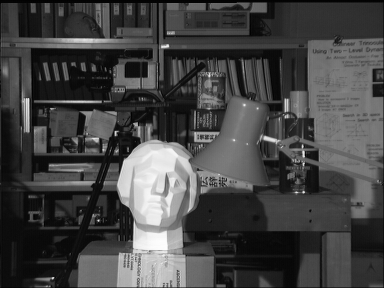
\includegraphics[width=\textwidth]{figures/tsukubaL.jpg}
		\caption{Left Tsukuba Grayscale Image}
		\label{fig:tsukubaL}
	\end{subfigure}
	\begin{subfigure}{0.45\textwidth}
		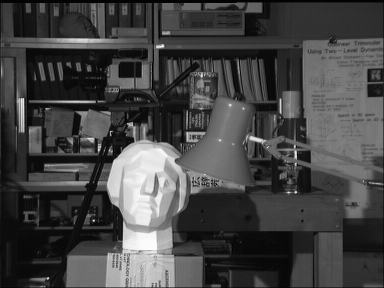
\includegraphics[width=\textwidth]{figures/tsukubaR.jpg}
		\caption{Right Tsukuba Grayscale Image}
		\label{fig:tsukubaR}
	\end{subfigure}
	\\
	\begin{subfigure}{0.45\textwidth}
		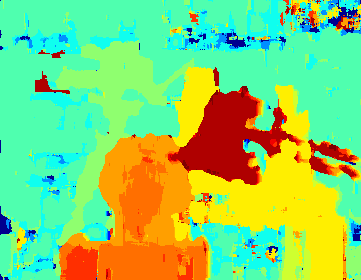
\includegraphics[width=\textwidth]{figures/tsukuba_c_9x9.png}
		\caption{C 9x9 Disparity Map}
		\label{fig:tsukubaC9x9}
	\end{subfigure}
	\begin{subfigure}{0.45\textwidth}
		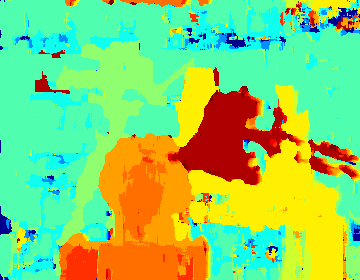
\includegraphics[width=\textwidth]{figures/tsukuba_9x9_fpga.png}
		\caption{FPGA 9x9 Disparity Map}
		\label{fig:tsukubaFPGA9x9}
	\end{subfigure}
	\\
	\begin{subfigure}{0.45\textwidth}
		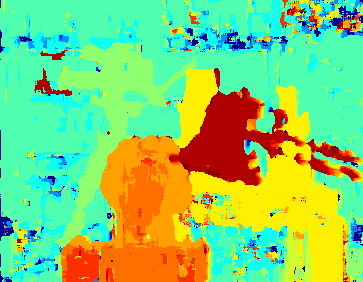
\includegraphics[width=\textwidth]{figures/tsukuba_c_7x7.png}
		\caption{C 7x7 Disparity Map}
		\label{fig:tsukubaC7x7}
	\end{subfigure}
	\begin{subfigure}{0.45\textwidth}
		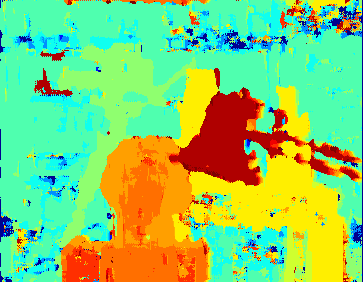
\includegraphics[width=\textwidth]{figures/tsukuba_7x7_fpga.png}
		\caption{FPGA 7x7 Disparity Map}
		\label{fig:tsukubaFPGA7x7}
	\end{subfigure}
	\captionfonts
	\caption{Disparity map comparison of the Tskukuba image pair~\cite{middlebury}.}
	\label{fig:tsukubaDispMap}
\end{center}
\end{figure}

\subsection{Venus}
\label{sec:venus}

In Figure~\ref{fig:venusL} and Figure~\ref{fig:venusR}, the Venus image pair is shown. In the image pair, the newspaper articles are flat and slanted, relative to the cameras. This gradual slope, also present in the background, can be difficult for the SAD algorithm to deal with; however, the algorithm is still able to give a fairly accurate representation of the depth in the image. It also causes the gradient pattern shown in the disparity maps. The 7x7 window depth maps have more noise than the 9x9 window depth maps.

For Venus, the FPGA version has a simulated runtime of 21.27 and 30.58 frames per second for the 9x9 and 7x7 window implementations, respectively, from Tbl.~\ref{table:tb_9x9} and Tbl.~\ref{table:tb_7x7}. As shown in Tbl.~\ref{table:runtimeComp}, the C code processed the images serially, which took 2.1681 seconds for the 9x9 window with a disparity range of 16. The 7x7 window implementation in C with a disparity range of 16 took 1.3438 seconds to complete.

\begin{figure}
\begin{center}
	\begin{subfigure}{0.45\textwidth}
		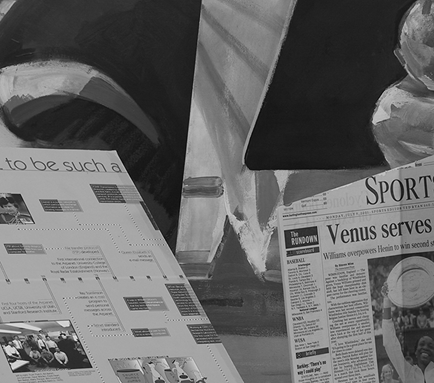
\includegraphics[width=\textwidth]{figures/venusL.png}
		\caption{Left Venus Grayscale Image}
		\label{fig:venusL}
	\end{subfigure}
	\begin{subfigure}{0.45\textwidth}
		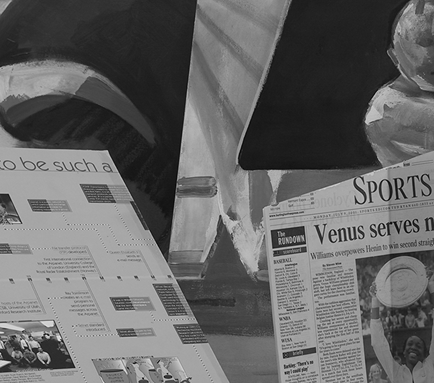
\includegraphics[width=\textwidth]{figures/venusR.png}
		\caption{Right Venus Grayscale Image}
		\label{fig:venusR}
	\end{subfigure}
	\\
	\begin{subfigure}{0.45\textwidth}
		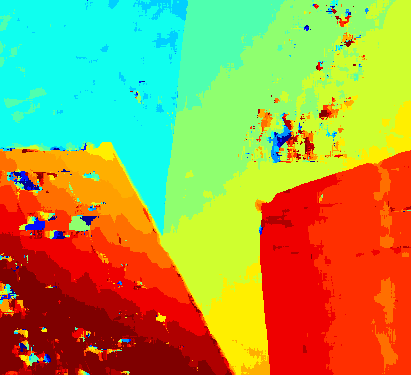
\includegraphics[width=\textwidth]{figures/venus_c_9x9.png}
		\caption{C 9x9 Disparity Map}
		\label{fig:venusC9x9}
	\end{subfigure}
	\begin{subfigure}{0.45\textwidth}
		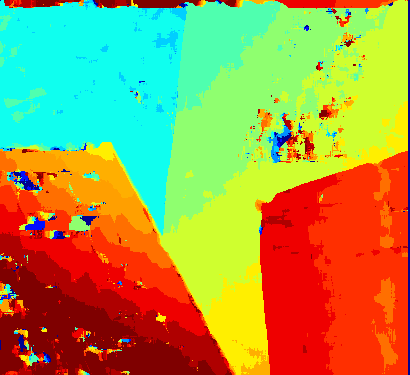
\includegraphics[width=\textwidth]{figures/venus_9x9_fpga.png}
		\caption{FPGA 9x9 Disparity Map}
		\label{fig:venusFPGA9x9}
	\end{subfigure}
	\\
	\begin{subfigure}{0.45\textwidth}
		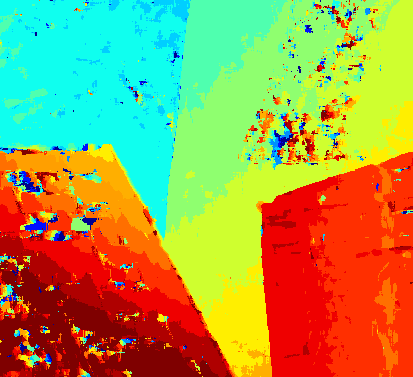
\includegraphics[width=\textwidth]{figures/venus_c_7x7.png}
		\caption{C 7x7 Disparity Map}
		\label{fig:venusC7x7}
	\end{subfigure}
	\begin{subfigure}{0.45\textwidth}
		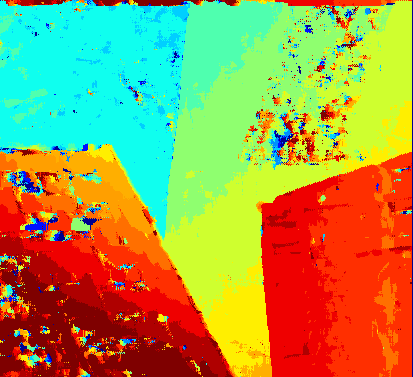
\includegraphics[width=\textwidth]{figures/venus_7x7_fpga.png}
		\caption{FPGA 7x7 Disparity Map}
		\label{fig:venusFPGA7x7}
	\end{subfigure}
	\captionfonts
	\caption{Disparity map comparison of the Venus image pair~\cite{middlebury}.}
	\label{fig:venusDispMap}
\end{center}
\end{figure}


\subsection{Cones}
\label{sec:cones}

In Figure~\ref{fig:conesL} and Figure~\ref{fig:conesR}, the Venus image pair is shown. Figure~\ref{fig:conesDispMap} shows the issue of objects in an image pair being too close to the stereo cameras. The closer an object is to the stereo cameras, the greater its disparity value will be. Using the SAD algorithm with a 9x9 window and a disparity range of 60 (as opposed to the range of 16 used on the FPGA board) produces the results in Figure~\ref{fig:conesMatlab}. When the disparity range is not high enough, the disparity map in Figure~\ref{fig:conesPy} is produced.

\begin{figure}
\begin{center}
	\begin{subfigure}{0.45\textwidth}
		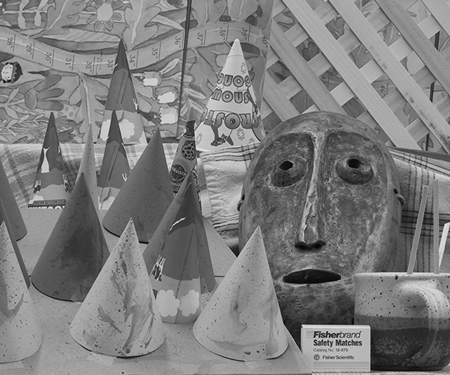
\includegraphics[width=\textwidth]{figures/conesL.png}
		\caption{Left Cones Grayscale Image}
		\label{fig:conesL}
	\end{subfigure}
	\begin{subfigure}{0.45\textwidth}
		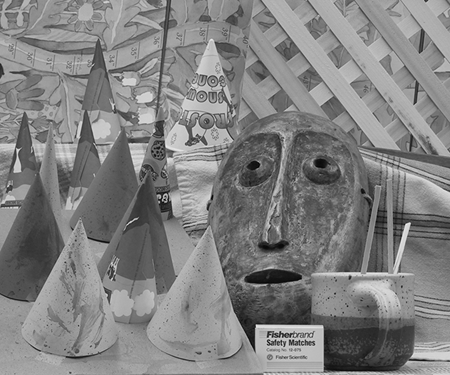
\includegraphics[width=\textwidth]{figures/conesR.png}
		\caption{Right Cones Grayscale Image}
		\label{fig:conesR}
	\end{subfigure}
	\\
	\begin{subfigure}{0.45\textwidth}
		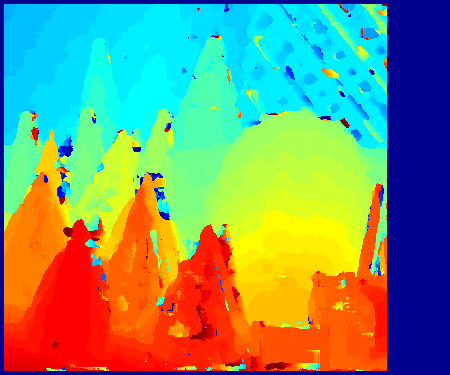
\includegraphics[width=\textwidth]{figures/cones_9x9_matlab_0-59.png}
		\caption{9x9 at Disparity Range of 60 ~\cite{matlab}}
		\label{fig:conesMatlab}
	\end{subfigure}
	\begin{subfigure}{0.45\textwidth}
		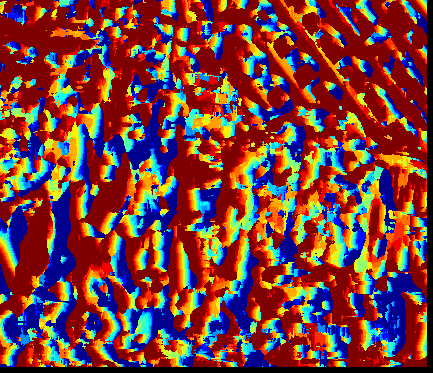
\includegraphics[width=\textwidth]{figures/cones_9x9_python3.png}
		\caption{9x9 at Disparity Range of 16}
		\label{fig:conesPy}
	\end{subfigure}
	\captionfonts
	\caption{Disparity map comparison of the Cones image pair ~\cite{middlebury}.}
	\label{fig:conesDispMap}
\end{center}
\end{figure}




